\documentclass{article}
\usepackage[utf8]{inputenc}
\usepackage{amstext}
\usepackage{amsmath} 
\usepackage{mathpazo}
\usepackage{graphicx} 
\usepackage{float} 
\usepackage{caption} 
\usepackage{epstopdf} 
\usepackage{hyperref}
\usepackage{varioref} 
\usepackage{fancyref}
\usepackage[section]{placeins} 
\usepackage{perpage}
\usepackage[margin=1in, paperwidth=8.5in, paperheight=11in]{geometry} 
\MakeSorted{figure} 
\usepackage{natbib}
\usepackage{graphicx}
\usepackage{xcolor}
\usepackage{listings}
\usepackage{minted}
\usepackage{subcaption}
\usepackage{eso-pic}
\usepackage{tikz}
\usepackage[american]{circuitikz}
\usepackage[font=small,labelfont=bf]{caption}

\title{ENGR2420 Lab 6 : Series/Parallel MOS Networks and MOS Current Dividers}
\author{Abigail Fry\\Anusha Datar\\ Vienna Scheyer}
\date{April 8, 2019}

\begin{document}

\maketitle

\section{Experiment One : Transistor Matching}
In the first experiment, we measured the change in the channel current as a function of gate voltage for each of the nMOS transistors on an ALD1106 transistor array. We connected the drain to $V_{dd}$, varied the input voltage at the gate, and measured the output current from source to ground. 
\begin{figure}[H]   
  \begin{center}       
  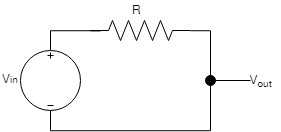
\includegraphics[scale = 0.5]{images/exp1_schematic.jpg}
  \caption{Schematic for the circuits used to measure the current response to changes in gate voltage for nMOS transistors.}   
  \label{fig:exp1_sch}
  \end{center}
\end{figure}

\subsection{Results}
We used the EKV model to determine values of the saturation current ($I_s$), divider ratio, $\kappa$, and the threshold voltage, $V_{T0}$ for each transistor. Figure 2 shows these values.

\begin{figure}[H]   
  \begin{center}      
  \includegraphics[scale = 0.4]{images/EKV_table.PNG}
  \caption{Values for $I_s$, $\kappa$, and $V_{t0}$ from the EKV model.}
  \end{center}
\end{figure}

We plotted the experimental and theoretical current response to gate voltage for each transistor on semilogarithmic axes, as shown in Figure 3.

\begin{figure}[H]   
  \begin{center}      
  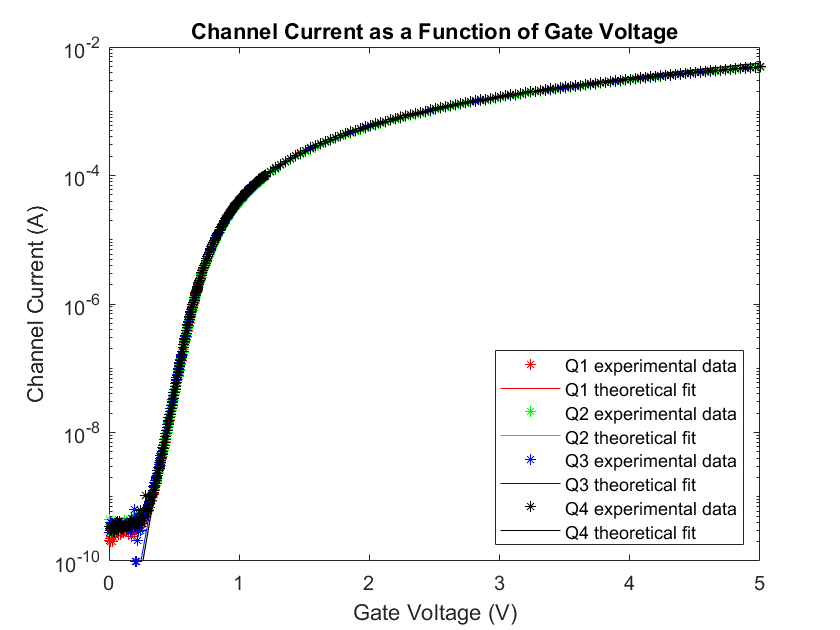
\includegraphics[scale = 0.6]{images/Exp1_EKV.png}
  \caption{Channel current as a function of gate voltage for four different transistors on an ALD1106 chip.}
  \label{fig:exp1_plot1}
  \end{center}
\end{figure}

We also plotted the percentage difference between each transistor’s channel current and the mean value of all four channel currents as a function of the mean value of all four channel currents as shown in Figure 4.

\begin{figure}[H]
  \begin{center}       
  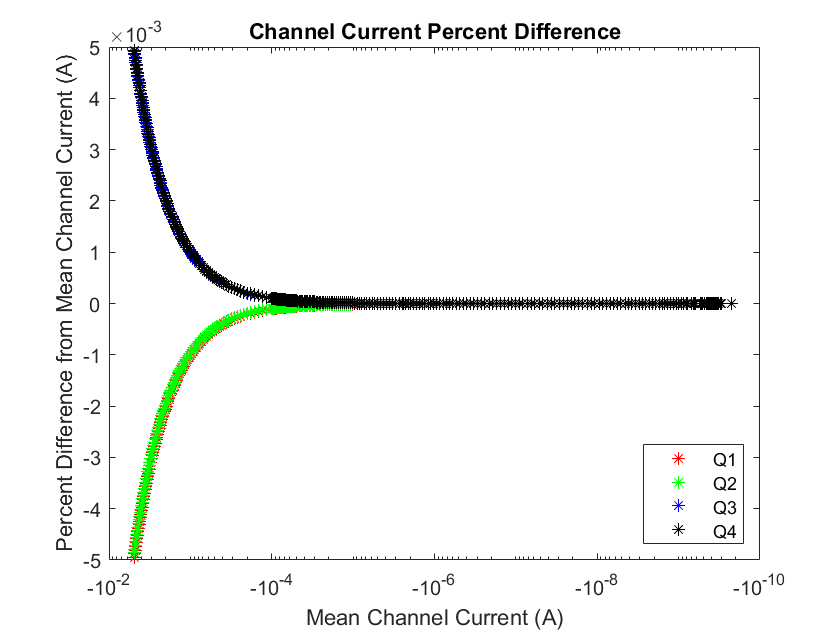
\includegraphics[scale = 0.6]{images/percent_diff.png}
  \label{fig:exp1_plot2}
  \caption{Percentage difference between each transistor's channel current and the mean value of all four channel currents as a function of the mean channel current for four different transistors on an ALD1106 chip.}
  \end{center}
\end{figure}
\subsection{Analysis}
By leveraging the EKV model and assuming that the channel current is equal to the saturation current, we determined appropriate values for $I_s$, $\kappa$, and $V_{T0}$.
Then we used the following equation to calculate a theoretical fit for the channel current of each transistor
\begin{center}
 $I_{sat} = I_{s}log^{2}{(1 + e^{\frac{\kappa(V_G - V_{T0}) - V_S)}{2U_T}}})$
\end{center}

Then we plotted experimental and theoretical fits on semilog y axes. The experimentally collected data matches the theoretical fit very well. You can see this in Figure 4 where we show the percent difference between each transistor's channel current and the mean current of all of the transistors is quite high. At low gate voltages, the percent difference is quite high. This might be due to error in measurement at very small currents. The percent difference quickly approaches zero, which is what we would expect for well matched transistors.

\subsection{Discussion}
The transistors match each other quite well. At low currents, the percent difference is non-zero than zero (0.005\%), and the percent difference quickly goes to zero. The devices match better in saturation mode.

\section{Experiment Two : MOS Transistors in Series and Parallel}
In experiment two, we measured the channel current as a function of gate voltage for $V_{DS}$ = $10 mV$ and $V_{DS}$ = $V_{dd}$ for one nMOS transistor. Then, we measured channel current as a function of gate voltage at both levels of $V_{DS}$ for two nMOS transistors in series and two nMOS transistors in parallel.
\begin{figure}[H]   
  \begin{center}       
  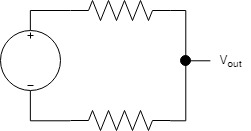
\includegraphics[scale = 0.5]{images/exp2_schematic.jpg}
  \caption{Schematics for the channel current measurement for a single device, transistors in series, and transistors in parallel.}
  \label{fig:exp2_sch}
  \end{center}
\end{figure}

\subsection{Results}
We can plot the relationship between gate voltage and channel current for each $V_{DS}$ value and each configuration (single, series, and parallel) on semilogarithmic axes.
\begin{figure}[H]   
  \begin{center}      
  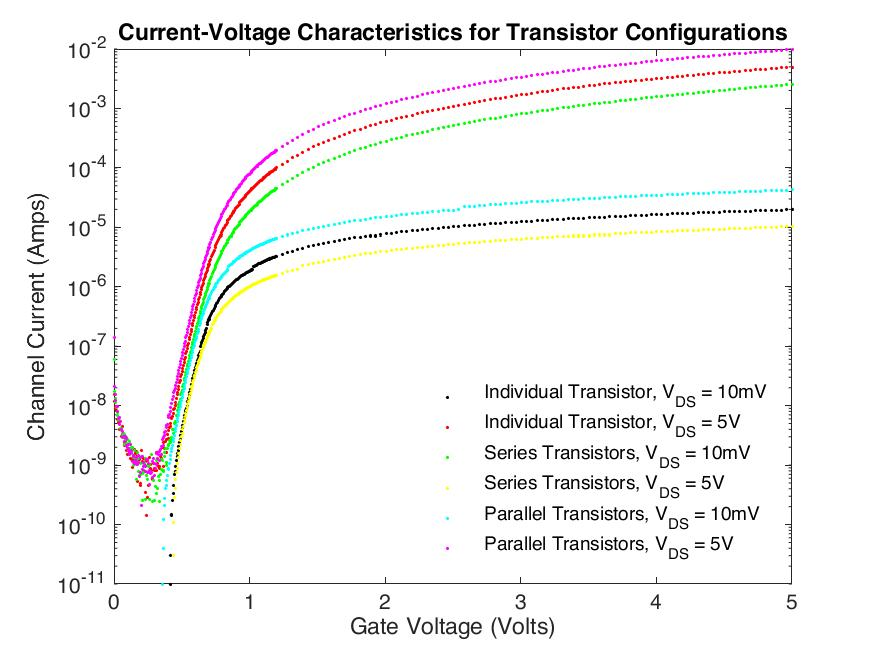
\includegraphics[scale = 0.4]{images/exp2plot1.jpg}
  \caption{Plot of channel current as a function of gate voltage for each device configuration and $V_{DS}$ value.}
  \label{fig:exp2_plot1}
  \end{center}
\end{figure}

We can also plot the ratio of the value of the channel current measurement for the series transistors and the channel current value of the single transistor.

\begin{figure}[H]   
    \begin{center}
  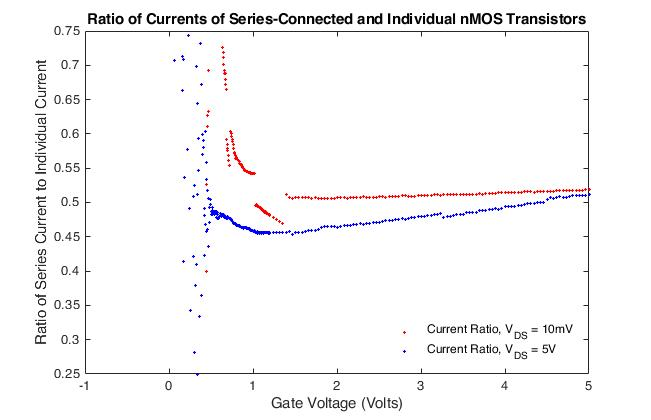
\includegraphics[scale = 0.4]{images/exp2plot2.jpg}
  \caption{Plot of the ratio between the series channel current measurement and the individual channel current measurement.}
  \label{fig:exp2_plot2}
    \end{center}

\end{figure}

Lastly, we can plot the ratio of the value of the channel current measurement for the parallel transistors and the channel current value of the single transistor
\begin{figure}[H]   
  \begin{center}       
  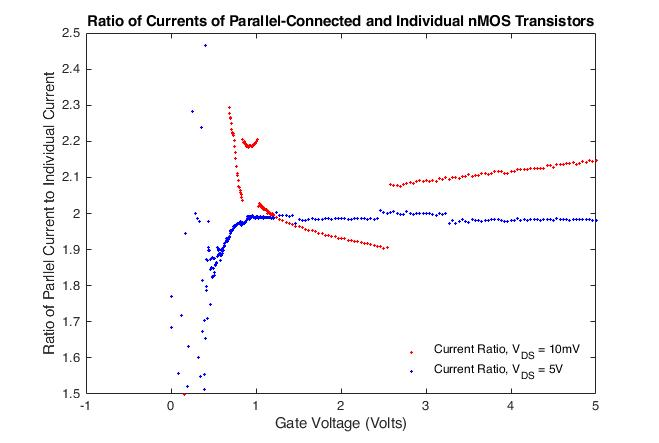
\includegraphics[scale = 0.4]{images/exp2plot3.jpg}
  \caption{Plot of the ratio between the parallel channel current measurement and the individual channel current measurement.}
  \label{fig:exp2_plot3}
  \end{center}
\end{figure}

\subsection{Analysis}
In theory, the value of the channel current for the transistors in series should be equal to half the value of the channel current for the individual transistor. Meanwhile, the value of the channel current for the transistors in parallel should be equal to double the value of the channel current for the individual transistor. 
\\
\newline
In practice, we measured the current values for the individual transistor, the series configuration, and the parallel configuration. Then, we used MATLAB's $polyfit$ function to determine the overall value of the ratio. Based on that, we found that the value of the current ratio for the series configuration is 0.4999 when the $V_{DS}$ is equal to 5V and 0.549 when the $V_{DS}$ is equal to 0.01V. For the parallel configuration, the current ratio is 2.1501 when the $V_{DS}$ is equal to 5V and 1.98311 when the $V_{DS}$ is equal to 0.01V.

Based on the expected value of 0.5 for the series ratio and 2 for the parallel ratio, we can determine the percent error by taking the quotient of the difference of the experimental and theoretical values and the theoretical values. We found that the value of the percent error for the series configuration is 0.0002\% when the $V_{DS}$ is equal to 5V and 0.0098\% when the $V_{DS}$ is equal to 0.01V. For the parallel configuration, the percent difference is 7.505\% when the $V_{DS}$ is equal to 5V and 0.00845\% when the $V_{DS}$ is equal to 0.01V.

Most of the errors, except for the one on the parallel transistor configuration with the 5 Volt $V_{DS}$ are fairly trivial. The one larger error likely can be attributed to the large variations present at low current where the data points are over sampled.
\subsection{Discussion}
While the average value of the ratio of the channel current of the series transistors is approximately equal to the expected value, the ratio is definitely not consistently constant at the expected value of the ratio. This is also the case for the parallel transistors. Instead, the ratio varies based on the region of operation of the transistor: when in the Ohmic region, the ratio is highly divergent from the expected value, and when in the saturation region, the ratio is much more even and close to the expected value. In the region where the transistors behave as expected, the series/parallel equivalences are a useful framework for studying and characterizing transistor behavior. Outside of these regions, they are a lot less useful, but the ratio is still within small integer values and may be appropriate in some applications. 


\section{Experiment Three : MOS Current Dividers}
In experiment three, we measured the channel current as a function of input current for two different MOS current dividers : one where current is sunk from the source measured at the drain and one where current is sourced at the drain and measured at the source.  For both current dividers, we swept current from 0 to 20 mA and set the gate voltage to $V_{dd}$ and the source voltage to ground.
\begin{figure}[H]   
  \begin{center}       
  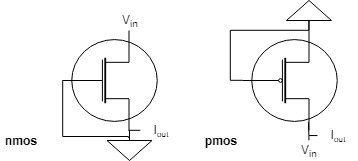
\includegraphics[scale = 0.5]{images/exp3_schematic.jpg}
  \caption{Schematics for the two MOS current dividers studied in this experiment.}
  \label{fig:exp2_sch}
  \end{center}
\end{figure}

\subsection{Results}
First, we plotted the experimental and theoretical input current vs. output current for the parallel current divider seen in Figure 10 on linear axes.
\begin{figure}[H]   
  \begin{center}      
  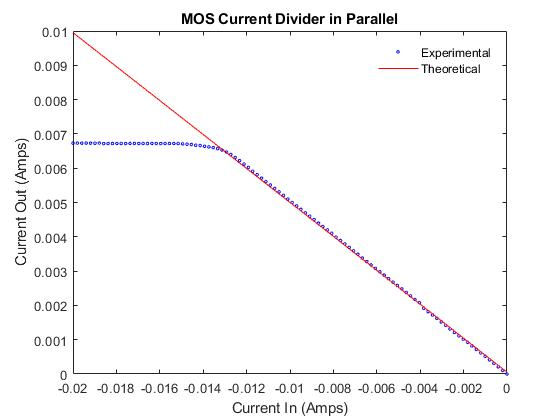
\includegraphics[scale = 0.6]{images/3_parallel.jpg}
  \caption{Input current vs. output current for parallel nMOS current divider where the
input current is sunk from the source and the output current is measured at the drains}
  \label{fig:exp3_parallel}
  \end{center}
\end{figure}
Then, we plotted the experimental and theoretical input current vs. output current for the series current divider seen in Figure 11 on linear axes.  
\begin{figure}[H]   
  \begin{center}      
  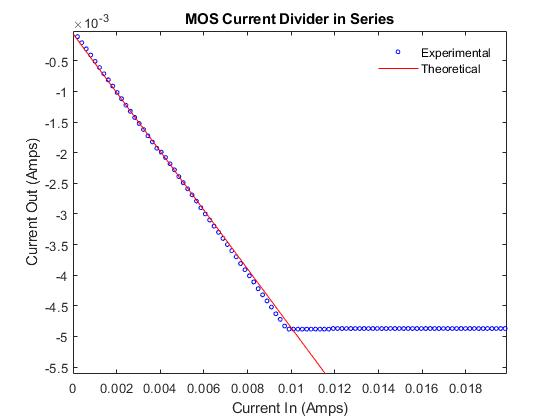
\includegraphics[scale = 0.6]{images/3_series.jpg}
  \caption{Input current vs. output current for series nMOS current divider where the input current is sourced into the drains and the output currents are taken at
the sources.}
  \label{fig:exp3_series}
  \end{center}
\end{figure}

\subsection{Analysis}
To find the current divider ratio (which is dimensionless), we used MATLAB's $polyfit$ function on the experimental data where the slope of the the line was not 0.  The slope of this region is the value of the divider ratio. 

The theoretical current divider ratio for both current dividers can be found using Kirchhoff’s Current Law (KCL) implies that 
\begin{center}
$I_{in} =
I_{1} + I_{2}$
\end{center}
For matched transistors like the ones in the chip we used, $I_{1}$ and $I_{2}$ are equivalent so the expected current divider ratio is
\begin{center}
$\frac{I_{1}}{I_{in}} = \frac{1}{2}$
\end{center}
 for both current dividers when $I_{1}$ is the measured output current.  The experimental value for the current divider of parallel nMOS transistors is -0.4949 and the theoretical value is -.5.  The experimental value for the current divider of series nMOS transistors is -0.4798 and the theoretical value is -.5. To calculate percent error of the experimental value, we used the following equation 
\begin{center}
 
Percent Error= $\frac{|(Theoretical-Experimental|}{Experimental}\times 100$


\end{center}
The percent error for the parallel nMOS current divider ratio is 1.02\% and the percent error for the series nMOS current divdier is 4.04\%.

\subsection{Discussion}
The ideal current divider ratio for both circuits is equal to $1/2$ from the current law analysis done in the pre-lab and in section 3.2.  In the experimental case, both current dividers had very similar ratios to the expected theoretical ratio.  The parallel nMOS current divider had a percent error of 1.02\%.  The series nMOS current divider had a percent error 4.04\%.  This error can be attributed to minute manufacturing disparities between the 2 transistors that were in array we used.

\end{document}
